\documentclass[]{article}
\usepackage{lmodern}
\usepackage{amssymb,amsmath}
\usepackage{ifxetex,ifluatex}
\usepackage{fixltx2e} % provides \textsubscript
\ifnum 0\ifxetex 1\fi\ifluatex 1\fi=0 % if pdftex
  \usepackage[T1]{fontenc}
  \usepackage[utf8]{inputenc}
\else % if luatex or xelatex
  \ifxetex
    \usepackage{mathspec}
  \else
    \usepackage{fontspec}
  \fi
  \defaultfontfeatures{Ligatures=TeX,Scale=MatchLowercase}
\fi
% use upquote if available, for straight quotes in verbatim environments
\IfFileExists{upquote.sty}{\usepackage{upquote}}{}
% use microtype if available
\IfFileExists{microtype.sty}{%
\usepackage{microtype}
\UseMicrotypeSet[protrusion]{basicmath} % disable protrusion for tt fonts
}{}
\usepackage[margin=1in]{geometry}
\usepackage{hyperref}
\hypersetup{unicode=true,
            pdftitle={Data Analysis},
            pdfauthor={Sridhar},
            pdfborder={0 0 0},
            breaklinks=true}
\urlstyle{same}  % don't use monospace font for urls
\usepackage{color}
\usepackage{fancyvrb}
\newcommand{\VerbBar}{|}
\newcommand{\VERB}{\Verb[commandchars=\\\{\}]}
\DefineVerbatimEnvironment{Highlighting}{Verbatim}{commandchars=\\\{\}}
% Add ',fontsize=\small' for more characters per line
\usepackage{framed}
\definecolor{shadecolor}{RGB}{248,248,248}
\newenvironment{Shaded}{\begin{snugshade}}{\end{snugshade}}
\newcommand{\KeywordTok}[1]{\textcolor[rgb]{0.13,0.29,0.53}{\textbf{#1}}}
\newcommand{\DataTypeTok}[1]{\textcolor[rgb]{0.13,0.29,0.53}{#1}}
\newcommand{\DecValTok}[1]{\textcolor[rgb]{0.00,0.00,0.81}{#1}}
\newcommand{\BaseNTok}[1]{\textcolor[rgb]{0.00,0.00,0.81}{#1}}
\newcommand{\FloatTok}[1]{\textcolor[rgb]{0.00,0.00,0.81}{#1}}
\newcommand{\ConstantTok}[1]{\textcolor[rgb]{0.00,0.00,0.00}{#1}}
\newcommand{\CharTok}[1]{\textcolor[rgb]{0.31,0.60,0.02}{#1}}
\newcommand{\SpecialCharTok}[1]{\textcolor[rgb]{0.00,0.00,0.00}{#1}}
\newcommand{\StringTok}[1]{\textcolor[rgb]{0.31,0.60,0.02}{#1}}
\newcommand{\VerbatimStringTok}[1]{\textcolor[rgb]{0.31,0.60,0.02}{#1}}
\newcommand{\SpecialStringTok}[1]{\textcolor[rgb]{0.31,0.60,0.02}{#1}}
\newcommand{\ImportTok}[1]{#1}
\newcommand{\CommentTok}[1]{\textcolor[rgb]{0.56,0.35,0.01}{\textit{#1}}}
\newcommand{\DocumentationTok}[1]{\textcolor[rgb]{0.56,0.35,0.01}{\textbf{\textit{#1}}}}
\newcommand{\AnnotationTok}[1]{\textcolor[rgb]{0.56,0.35,0.01}{\textbf{\textit{#1}}}}
\newcommand{\CommentVarTok}[1]{\textcolor[rgb]{0.56,0.35,0.01}{\textbf{\textit{#1}}}}
\newcommand{\OtherTok}[1]{\textcolor[rgb]{0.56,0.35,0.01}{#1}}
\newcommand{\FunctionTok}[1]{\textcolor[rgb]{0.00,0.00,0.00}{#1}}
\newcommand{\VariableTok}[1]{\textcolor[rgb]{0.00,0.00,0.00}{#1}}
\newcommand{\ControlFlowTok}[1]{\textcolor[rgb]{0.13,0.29,0.53}{\textbf{#1}}}
\newcommand{\OperatorTok}[1]{\textcolor[rgb]{0.81,0.36,0.00}{\textbf{#1}}}
\newcommand{\BuiltInTok}[1]{#1}
\newcommand{\ExtensionTok}[1]{#1}
\newcommand{\PreprocessorTok}[1]{\textcolor[rgb]{0.56,0.35,0.01}{\textit{#1}}}
\newcommand{\AttributeTok}[1]{\textcolor[rgb]{0.77,0.63,0.00}{#1}}
\newcommand{\RegionMarkerTok}[1]{#1}
\newcommand{\InformationTok}[1]{\textcolor[rgb]{0.56,0.35,0.01}{\textbf{\textit{#1}}}}
\newcommand{\WarningTok}[1]{\textcolor[rgb]{0.56,0.35,0.01}{\textbf{\textit{#1}}}}
\newcommand{\AlertTok}[1]{\textcolor[rgb]{0.94,0.16,0.16}{#1}}
\newcommand{\ErrorTok}[1]{\textcolor[rgb]{0.64,0.00,0.00}{\textbf{#1}}}
\newcommand{\NormalTok}[1]{#1}
\usepackage{graphicx,grffile}
\makeatletter
\def\maxwidth{\ifdim\Gin@nat@width>\linewidth\linewidth\else\Gin@nat@width\fi}
\def\maxheight{\ifdim\Gin@nat@height>\textheight\textheight\else\Gin@nat@height\fi}
\makeatother
% Scale images if necessary, so that they will not overflow the page
% margins by default, and it is still possible to overwrite the defaults
% using explicit options in \includegraphics[width, height, ...]{}
\setkeys{Gin}{width=\maxwidth,height=\maxheight,keepaspectratio}
\IfFileExists{parskip.sty}{%
\usepackage{parskip}
}{% else
\setlength{\parindent}{0pt}
\setlength{\parskip}{6pt plus 2pt minus 1pt}
}
\setlength{\emergencystretch}{3em}  % prevent overfull lines
\providecommand{\tightlist}{%
  \setlength{\itemsep}{0pt}\setlength{\parskip}{0pt}}
\setcounter{secnumdepth}{0}
% Redefines (sub)paragraphs to behave more like sections
\ifx\paragraph\undefined\else
\let\oldparagraph\paragraph
\renewcommand{\paragraph}[1]{\oldparagraph{#1}\mbox{}}
\fi
\ifx\subparagraph\undefined\else
\let\oldsubparagraph\subparagraph
\renewcommand{\subparagraph}[1]{\oldsubparagraph{#1}\mbox{}}
\fi

%%% Use protect on footnotes to avoid problems with footnotes in titles
\let\rmarkdownfootnote\footnote%
\def\footnote{\protect\rmarkdownfootnote}

%%% Change title format to be more compact
\usepackage{titling}

% Create subtitle command for use in maketitle
\newcommand{\subtitle}[1]{
  \posttitle{
    \begin{center}\large#1\end{center}
    }
}

\setlength{\droptitle}{-2em}

  \title{Data Analysis}
    \pretitle{\vspace{\droptitle}\centering\huge}
  \posttitle{\par}
    \author{Sridhar}
    \preauthor{\centering\large\emph}
  \postauthor{\par}
      \predate{\centering\large\emph}
  \postdate{\par}
    \date{28 January 2019}


\begin{document}
\maketitle

\begin{Shaded}
\begin{Highlighting}[]
\CommentTok{#install.packages("ggplot2")}
\CommentTok{#install.packages("ggvis")}
\CommentTok{#install.packages("mice")}
\KeywordTok{library}\NormalTok{(ggplot2)}
\KeywordTok{library}\NormalTok{(ggvis)}
\end{Highlighting}
\end{Shaded}

\begin{verbatim}
## 
## Attaching package: 'ggvis'
\end{verbatim}

\begin{verbatim}
## The following object is masked from 'package:ggplot2':
## 
##     resolution
\end{verbatim}

\begin{Shaded}
\begin{Highlighting}[]
\KeywordTok{library}\NormalTok{(knitr)}
\KeywordTok{library}\NormalTok{(mice)}
\end{Highlighting}
\end{Shaded}

\begin{verbatim}
## Loading required package: lattice
\end{verbatim}

\begin{verbatim}
## 
## Attaching package: 'mice'
\end{verbatim}

\begin{verbatim}
## The following objects are masked from 'package:base':
## 
##     cbind, rbind
\end{verbatim}

\begin{Shaded}
\begin{Highlighting}[]
\KeywordTok{library}\NormalTok{(caret)}
\KeywordTok{library}\NormalTok{(doParallel) }
\end{Highlighting}
\end{Shaded}

\begin{verbatim}
## Loading required package: foreach
\end{verbatim}

\begin{verbatim}
## Loading required package: iterators
\end{verbatim}

\begin{verbatim}
## Loading required package: parallel
\end{verbatim}

\subsection{Load the Data}\label{load-the-data}

Breast Cancer Wisconsin(Diagnosis) data is loaded and the column names
are defined based on the attribute information.

\subsubsection{Dataset 1}\label{dataset-1}

The outcome variable is the ``classes'' and it has following category of
data

\begin{itemize}
\tightlist
\item
  Malignant or
\item
  Benign breast mass
\end{itemize}

The phenotypes for characterization are * Sample ID (code number) *
Clump thickness * Uniformity of cell size * Uniformity of cell shape *
Marginal adhesion * Single epithelial cell size * Number of bare nuclei
* Bland chromatin * Number of normal nuclei * Mitosis * Classes,
i.e.~diagnosis

\begin{Shaded}
\begin{Highlighting}[]
\NormalTok{diagnosis_data <-}\StringTok{ }\KeywordTok{read.csv}\NormalTok{(}\StringTok{"~/Desktop/BreastCancer/Data/breast-cancer-wisconsin.data.csv"}\NormalTok{, }\DataTypeTok{header =} \OtherTok{FALSE}\NormalTok{)}
\KeywordTok{colnames}\NormalTok{(diagnosis_data) <-}\StringTok{ }\KeywordTok{c}\NormalTok{(}\StringTok{"sample_code_number"}\NormalTok{, }\StringTok{"clump_thickness"}\NormalTok{, }\StringTok{"uniformity_of_cell_size"}\NormalTok{, }\StringTok{"uniformity_of_cell_shape"}\NormalTok{, }\StringTok{"marginal_adhesion"}\NormalTok{, }\StringTok{"single_epithelial_cell_size"}\NormalTok{, }
                       \StringTok{"bare_nuclei"}\NormalTok{, }\StringTok{"bland_chromatin"}\NormalTok{, }\StringTok{"normal_nucleoli"}\NormalTok{, }\StringTok{"mitosis"}\NormalTok{, }\StringTok{"classes"}\NormalTok{)}
\end{Highlighting}
\end{Shaded}

\begin{Shaded}
\begin{Highlighting}[]
\CommentTok{# impute missing data}

\NormalTok{diagnosis_data[,}\DecValTok{2}\OperatorTok{:}\DecValTok{10}\NormalTok{] <-}\StringTok{ }\KeywordTok{apply}\NormalTok{(diagnosis_data[, }\DecValTok{2}\OperatorTok{:}\DecValTok{10}\NormalTok{], }\DecValTok{2}\NormalTok{, }\ControlFlowTok{function}\NormalTok{(x) }\KeywordTok{as.numeric}\NormalTok{(}\KeywordTok{as.character}\NormalTok{(x)))}
\end{Highlighting}
\end{Shaded}

\begin{verbatim}
## Warning in FUN(newX[, i], ...): NAs introduced by coercion
\end{verbatim}

\begin{Shaded}
\begin{Highlighting}[]
\NormalTok{dataset_impute <-}\StringTok{ }\KeywordTok{mice}\NormalTok{(diagnosis_data[, }\DecValTok{2}\OperatorTok{:}\DecValTok{10}\NormalTok{],  }\DataTypeTok{print =} \OtherTok{FALSE}\NormalTok{)}
\NormalTok{diagnosis_data <-}\StringTok{ }\KeywordTok{cbind}\NormalTok{(diagnosis_data[, }\DecValTok{11}\NormalTok{, }\DataTypeTok{drop =} \OtherTok{FALSE}\NormalTok{], mice}\OperatorTok{::}\KeywordTok{complete}\NormalTok{(dataset_impute, }\DecValTok{1}\NormalTok{))}

\NormalTok{diagnosis_data}\OperatorTok{$}\NormalTok{classes <-}\StringTok{ }\KeywordTok{as.factor}\NormalTok{(diagnosis_data}\OperatorTok{$}\NormalTok{classes)}

\CommentTok{# how many benign and malignant cases are there?}
\KeywordTok{summary}\NormalTok{(diagnosis_data}\OperatorTok{$}\NormalTok{classes)}
\end{Highlighting}
\end{Shaded}

\begin{verbatim}
##   2   4 
## 458 241
\end{verbatim}

The data is presented below.

\begin{Shaded}
\begin{Highlighting}[]
\KeywordTok{head}\NormalTok{(diagnosis_data)}
\end{Highlighting}
\end{Shaded}

\begin{verbatim}
##   classes clump_thickness uniformity_of_cell_size uniformity_of_cell_shape
## 1       2               5                       1                        1
## 2       2               5                       4                        4
## 3       2               3                       1                        1
## 4       2               6                       8                        8
## 5       2               4                       1                        1
## 6       4               8                      10                       10
##   marginal_adhesion single_epithelial_cell_size bare_nuclei
## 1                 1                           2           1
## 2                 5                           7          10
## 3                 1                           2           2
## 4                 1                           3           4
## 5                 3                           2           1
## 6                 8                           7          10
##   bland_chromatin normal_nucleoli mitosis
## 1               3               1       1
## 2               3               2       1
## 3               3               1       1
## 4               3               7       1
## 5               3               1       1
## 6               9               7       1
\end{verbatim}

The properties of data are given,

\begin{Shaded}
\begin{Highlighting}[]
\KeywordTok{str}\NormalTok{(diagnosis_data)}
\end{Highlighting}
\end{Shaded}

\begin{verbatim}
## 'data.frame':    699 obs. of  10 variables:
##  $ classes                    : Factor w/ 2 levels "2","4": 1 1 1 1 1 2 1 1 1 1 ...
##  $ clump_thickness            : num  5 5 3 6 4 8 1 2 2 4 ...
##  $ uniformity_of_cell_size    : num  1 4 1 8 1 10 1 1 1 2 ...
##  $ uniformity_of_cell_shape   : num  1 4 1 8 1 10 1 2 1 1 ...
##  $ marginal_adhesion          : num  1 5 1 1 3 8 1 1 1 1 ...
##  $ single_epithelial_cell_size: num  2 7 2 3 2 7 2 2 2 2 ...
##  $ bare_nuclei                : num  1 10 2 4 1 10 10 1 1 1 ...
##  $ bland_chromatin            : num  3 3 3 3 3 9 3 3 1 2 ...
##  $ normal_nucleoli            : num  1 2 1 7 1 7 1 1 1 1 ...
##  $ mitosis                    : num  1 1 1 1 1 1 1 1 5 1 ...
\end{verbatim}

\subsubsection{Dataset 2}\label{dataset-2}

The outcome variable is the ``classes'' and it has following category of
data Attribute Information:

\begin{enumerate}
\def\labelenumi{\arabic{enumi})}
\tightlist
\item
  ID number
\item
  Diagnosis (M = malignant, B = benign) 3-32)
\end{enumerate}

Ten real-valued features are computed for each cell nucleus:

\begin{enumerate}
\def\labelenumi{\alph{enumi})}
\tightlist
\item
  radius (mean of distances from center to points on the perimeter)
\item
  texture (standard deviation of gray-scale values)
\item
  perimeter
\item
  area
\item
  smoothness (local variation in radius lengths)
\item
  compactness (perimeter\^{}2 / area - 1.0)
\item
  concavity (severity of concave portions of the contour)
\item
  concave points (number of concave portions of the contour)
\item
  symmetry
\item
  fractal dimension (``coastline approximation'' - 1)
\end{enumerate}

\begin{Shaded}
\begin{Highlighting}[]
\NormalTok{diagnosis_data_}\DecValTok{2}\NormalTok{ <-}\StringTok{ }\KeywordTok{read.csv}\NormalTok{(}\StringTok{"~/Desktop/BreastCancer/Data/wdbc.data.csv"}\NormalTok{, }\DataTypeTok{header =} \OtherTok{FALSE}\NormalTok{)}

\NormalTok{phenotypes <-}\StringTok{ }\KeywordTok{rep}\NormalTok{(}\KeywordTok{c}\NormalTok{(}\StringTok{"radius"}\NormalTok{, }\StringTok{"texture"}\NormalTok{, }\StringTok{"perimeter"}\NormalTok{, }\StringTok{"area"}\NormalTok{, }\StringTok{"smoothness"}\NormalTok{, }\StringTok{"compactness"}\NormalTok{, }\StringTok{"concavity"}\NormalTok{, }\StringTok{"concave_points"}\NormalTok{, }\StringTok{"symmetry"}\NormalTok{, }\StringTok{"fractal_dimension"}\NormalTok{), }\DecValTok{3}\NormalTok{)}
\NormalTok{types <-}\StringTok{ }\KeywordTok{rep}\NormalTok{(}\KeywordTok{c}\NormalTok{(}\StringTok{"mean"}\NormalTok{, }\StringTok{"se"}\NormalTok{, }\StringTok{"largest_worst"}\NormalTok{), }\DataTypeTok{each =} \DecValTok{10}\NormalTok{)}

\KeywordTok{colnames}\NormalTok{(diagnosis_data_}\DecValTok{2}\NormalTok{) <-}\StringTok{ }\KeywordTok{c}\NormalTok{(}\StringTok{"ID"}\NormalTok{, }\StringTok{"diagnosis"}\NormalTok{, }\KeywordTok{paste}\NormalTok{(phenotypes, types, }\DataTypeTok{sep =} \StringTok{"_"}\NormalTok{))}
\KeywordTok{head}\NormalTok{(diagnosis_data_}\DecValTok{2}\NormalTok{)}
\end{Highlighting}
\end{Shaded}

\begin{verbatim}
##         ID diagnosis radius_mean texture_mean perimeter_mean area_mean
## 1   842302         M       17.99        10.38         122.80    1001.0
## 2   842517         M       20.57        17.77         132.90    1326.0
## 3 84300903         M       19.69        21.25         130.00    1203.0
## 4 84348301         M       11.42        20.38          77.58     386.1
## 5 84358402         M       20.29        14.34         135.10    1297.0
## 6   843786         M       12.45        15.70          82.57     477.1
##   smoothness_mean compactness_mean concavity_mean concave_points_mean
## 1         0.11840          0.27760         0.3001             0.14710
## 2         0.08474          0.07864         0.0869             0.07017
## 3         0.10960          0.15990         0.1974             0.12790
## 4         0.14250          0.28390         0.2414             0.10520
## 5         0.10030          0.13280         0.1980             0.10430
## 6         0.12780          0.17000         0.1578             0.08089
##   symmetry_mean fractal_dimension_mean radius_se texture_se perimeter_se
## 1        0.2419                0.07871    1.0950     0.9053        8.589
## 2        0.1812                0.05667    0.5435     0.7339        3.398
## 3        0.2069                0.05999    0.7456     0.7869        4.585
## 4        0.2597                0.09744    0.4956     1.1560        3.445
## 5        0.1809                0.05883    0.7572     0.7813        5.438
## 6        0.2087                0.07613    0.3345     0.8902        2.217
##   area_se smoothness_se compactness_se concavity_se concave_points_se
## 1  153.40      0.006399        0.04904      0.05373           0.01587
## 2   74.08      0.005225        0.01308      0.01860           0.01340
## 3   94.03      0.006150        0.04006      0.03832           0.02058
## 4   27.23      0.009110        0.07458      0.05661           0.01867
## 5   94.44      0.011490        0.02461      0.05688           0.01885
## 6   27.19      0.007510        0.03345      0.03672           0.01137
##   symmetry_se fractal_dimension_se radius_largest_worst
## 1     0.03003             0.006193                25.38
## 2     0.01389             0.003532                24.99
## 3     0.02250             0.004571                23.57
## 4     0.05963             0.009208                14.91
## 5     0.01756             0.005115                22.54
## 6     0.02165             0.005082                15.47
##   texture_largest_worst perimeter_largest_worst area_largest_worst
## 1                 17.33                  184.60             2019.0
## 2                 23.41                  158.80             1956.0
## 3                 25.53                  152.50             1709.0
## 4                 26.50                   98.87              567.7
## 5                 16.67                  152.20             1575.0
## 6                 23.75                  103.40              741.6
##   smoothness_largest_worst compactness_largest_worst
## 1                   0.1622                    0.6656
## 2                   0.1238                    0.1866
## 3                   0.1444                    0.4245
## 4                   0.2098                    0.8663
## 5                   0.1374                    0.2050
## 6                   0.1791                    0.5249
##   concavity_largest_worst concave_points_largest_worst
## 1                  0.7119                       0.2654
## 2                  0.2416                       0.1860
## 3                  0.4504                       0.2430
## 4                  0.6869                       0.2575
## 5                  0.4000                       0.1625
## 6                  0.5355                       0.1741
##   symmetry_largest_worst fractal_dimension_largest_worst
## 1                 0.4601                         0.11890
## 2                 0.2750                         0.08902
## 3                 0.3613                         0.08758
## 4                 0.6638                         0.17300
## 5                 0.2364                         0.07678
## 6                 0.3985                         0.12440
\end{verbatim}

\begin{Shaded}
\begin{Highlighting}[]
\KeywordTok{str}\NormalTok{(diagnosis_data_}\DecValTok{2}\NormalTok{)}
\end{Highlighting}
\end{Shaded}

\begin{verbatim}
## 'data.frame':    569 obs. of  32 variables:
##  $ ID                             : int  842302 842517 84300903 84348301 84358402 843786 844359 84458202 844981 84501001 ...
##  $ diagnosis                      : Factor w/ 2 levels "B","M": 2 2 2 2 2 2 2 2 2 2 ...
##  $ radius_mean                    : num  18 20.6 19.7 11.4 20.3 ...
##  $ texture_mean                   : num  10.4 17.8 21.2 20.4 14.3 ...
##  $ perimeter_mean                 : num  122.8 132.9 130 77.6 135.1 ...
##  $ area_mean                      : num  1001 1326 1203 386 1297 ...
##  $ smoothness_mean                : num  0.1184 0.0847 0.1096 0.1425 0.1003 ...
##  $ compactness_mean               : num  0.2776 0.0786 0.1599 0.2839 0.1328 ...
##  $ concavity_mean                 : num  0.3001 0.0869 0.1974 0.2414 0.198 ...
##  $ concave_points_mean            : num  0.1471 0.0702 0.1279 0.1052 0.1043 ...
##  $ symmetry_mean                  : num  0.242 0.181 0.207 0.26 0.181 ...
##  $ fractal_dimension_mean         : num  0.0787 0.0567 0.06 0.0974 0.0588 ...
##  $ radius_se                      : num  1.095 0.543 0.746 0.496 0.757 ...
##  $ texture_se                     : num  0.905 0.734 0.787 1.156 0.781 ...
##  $ perimeter_se                   : num  8.59 3.4 4.58 3.44 5.44 ...
##  $ area_se                        : num  153.4 74.1 94 27.2 94.4 ...
##  $ smoothness_se                  : num  0.0064 0.00522 0.00615 0.00911 0.01149 ...
##  $ compactness_se                 : num  0.049 0.0131 0.0401 0.0746 0.0246 ...
##  $ concavity_se                   : num  0.0537 0.0186 0.0383 0.0566 0.0569 ...
##  $ concave_points_se              : num  0.0159 0.0134 0.0206 0.0187 0.0188 ...
##  $ symmetry_se                    : num  0.03 0.0139 0.0225 0.0596 0.0176 ...
##  $ fractal_dimension_se           : num  0.00619 0.00353 0.00457 0.00921 0.00511 ...
##  $ radius_largest_worst           : num  25.4 25 23.6 14.9 22.5 ...
##  $ texture_largest_worst          : num  17.3 23.4 25.5 26.5 16.7 ...
##  $ perimeter_largest_worst        : num  184.6 158.8 152.5 98.9 152.2 ...
##  $ area_largest_worst             : num  2019 1956 1709 568 1575 ...
##  $ smoothness_largest_worst       : num  0.162 0.124 0.144 0.21 0.137 ...
##  $ compactness_largest_worst      : num  0.666 0.187 0.424 0.866 0.205 ...
##  $ concavity_largest_worst        : num  0.712 0.242 0.45 0.687 0.4 ...
##  $ concave_points_largest_worst   : num  0.265 0.186 0.243 0.258 0.163 ...
##  $ symmetry_largest_worst         : num  0.46 0.275 0.361 0.664 0.236 ...
##  $ fractal_dimension_largest_worst: num  0.1189 0.089 0.0876 0.173 0.0768 ...
\end{verbatim}

\begin{Shaded}
\begin{Highlighting}[]
\NormalTok{diagnosis_data_}\DecValTok{3}\NormalTok{ <-}\StringTok{ }\KeywordTok{read.csv}\NormalTok{(}\StringTok{"~/Desktop/BreastCancer/Data/wpbc.data.csv"}\NormalTok{, }\DataTypeTok{header =} \OtherTok{FALSE}\NormalTok{)}

\KeywordTok{colnames}\NormalTok{(diagnosis_data_}\DecValTok{3}\NormalTok{) <-}\StringTok{ }\KeywordTok{c}\NormalTok{(}\StringTok{"ID"}\NormalTok{, }\StringTok{"outcome"}\NormalTok{, }\StringTok{"time"}\NormalTok{, }\KeywordTok{paste}\NormalTok{(phenotypes, types, }\DataTypeTok{sep =} \StringTok{"_"}\NormalTok{), }\StringTok{"tumor_size"}\NormalTok{, }\StringTok{"lymph_node_status"}\NormalTok{)}
\NormalTok{diagnosis_data_}\DecValTok{3}\NormalTok{[diagnosis_data_}\DecValTok{3} \OperatorTok{==}\StringTok{ "?"}\NormalTok{] <-}\StringTok{ }\OtherTok{NA}
\KeywordTok{head}\NormalTok{(diagnosis_data_}\DecValTok{3}\NormalTok{)}
\end{Highlighting}
\end{Shaded}

\begin{verbatim}
##       ID outcome time radius_mean texture_mean perimeter_mean area_mean
## 1 119513       N   31       18.02        27.60         117.50    1013.0
## 2   8423       N   61       17.99        10.38         122.80    1001.0
## 3 842517       N  116       21.37        17.44         137.50    1373.0
## 4 843483       N  123       11.42        20.38          77.58     386.1
## 5 843584       R   27       20.29        14.34         135.10    1297.0
## 6 843786       R   77       12.75        15.29          84.60     502.7
##   smoothness_mean compactness_mean concavity_mean concave_points_mean
## 1         0.09489           0.1036         0.1086             0.07055
## 2         0.11840           0.2776         0.3001             0.14710
## 3         0.08836           0.1189         0.1255             0.08180
## 4         0.14250           0.2839         0.2414             0.10520
## 5         0.10030           0.1328         0.1980             0.10430
## 6         0.11890           0.1569         0.1664             0.07666
##   symmetry_mean fractal_dimension_mean radius_se texture_se perimeter_se
## 1        0.1865                0.06333    0.6249     1.8900        3.972
## 2        0.2419                0.07871    1.0950     0.9053        8.589
## 3        0.2333                0.06010    0.5854     0.6105        3.928
## 4        0.2597                0.09744    0.4956     1.1560        3.445
## 5        0.1809                0.05883    0.7572     0.7813        5.438
## 6        0.1995                0.07164    0.3877     0.7402        2.999
##   area_se smoothness_se compactness_se concavity_se concave_points_se
## 1   71.55      0.004433        0.01421      0.03233          0.009854
## 2  153.40      0.006399        0.04904      0.05373          0.015870
## 3   82.15      0.006167        0.03449      0.03300          0.018050
## 4   27.23      0.009110        0.07458      0.05661          0.018670
## 5   94.44      0.011490        0.02461      0.05688          0.018850
## 6   30.85      0.007775        0.02987      0.04561          0.013570
##   symmetry_se fractal_dimension_se radius_largest_worst
## 1     0.01694             0.003495                21.63
## 2     0.03003             0.006193                25.38
## 3     0.03094             0.005039                24.90
## 4     0.05963             0.009208                14.91
## 5     0.01756             0.005115                22.54
## 6     0.01774             0.005114                15.51
##   texture_largest_worst perimeter_largest_worst area_largest_worst
## 1                 37.08                  139.70             1436.0
## 2                 17.33                  184.60             2019.0
## 3                 20.98                  159.10             1949.0
## 4                 26.50                   98.87              567.7
## 5                 16.67                  152.20             1575.0
## 6                 20.37                  107.30              733.2
##   smoothness_largest_worst compactness_largest_worst
## 1                   0.1195                    0.1926
## 2                   0.1622                    0.6656
## 3                   0.1188                    0.3449
## 4                   0.2098                    0.8663
## 5                   0.1374                    0.2050
## 6                   0.1706                    0.4196
##   concavity_largest_worst concave_points_largest_worst
## 1                  0.3140                       0.1170
## 2                  0.7119                       0.2654
## 3                  0.3414                       0.2032
## 4                  0.6869                       0.2575
## 5                  0.4000                       0.1625
## 6                  0.5999                       0.1709
##   symmetry_largest_worst fractal_dimension_largest_worst tumor_size
## 1                 0.2677                         0.08113        5.0
## 2                 0.4601                         0.11890        3.0
## 3                 0.4334                         0.09067        2.5
## 4                 0.6638                         0.17300        2.0
## 5                 0.2364                         0.07678        3.5
## 6                 0.3485                         0.11790        2.5
##   lymph_node_status
## 1                 5
## 2                 2
## 3                 0
## 4                 0
## 5                 0
## 6                 0
\end{verbatim}

\begin{Shaded}
\begin{Highlighting}[]
\NormalTok{diagnosis_data_}\DecValTok{3}\NormalTok{[,}\DecValTok{3}\OperatorTok{:}\DecValTok{35}\NormalTok{] <-}\StringTok{ }\KeywordTok{apply}\NormalTok{(diagnosis_data_}\DecValTok{3}\NormalTok{[,}\DecValTok{3}\OperatorTok{:}\DecValTok{35}\NormalTok{], }\DecValTok{2}\NormalTok{, }\ControlFlowTok{function}\NormalTok{(x) }\KeywordTok{as.numeric}\NormalTok{(}\KeywordTok{as.character}\NormalTok{(x)))}
\NormalTok{dataset_impute <-}\StringTok{ }\KeywordTok{mice}\NormalTok{(diagnosis_data_}\DecValTok{3}\NormalTok{[,}\DecValTok{3}\OperatorTok{:}\DecValTok{35}\NormalTok{],  }\DataTypeTok{print =} \OtherTok{FALSE}\NormalTok{)}
\end{Highlighting}
\end{Shaded}

\begin{verbatim}
## Warning: Number of logged events: 25
\end{verbatim}

\begin{Shaded}
\begin{Highlighting}[]
\NormalTok{diagnosis_data_}\DecValTok{3}\NormalTok{ <-}\StringTok{ }\KeywordTok{cbind}\NormalTok{(diagnosis_data_}\DecValTok{3}\NormalTok{[, }\DecValTok{2}\NormalTok{, }\DataTypeTok{drop =} \OtherTok{FALSE}\NormalTok{], mice}\OperatorTok{::}\KeywordTok{complete}\NormalTok{(dataset_impute, }\DecValTok{1}\NormalTok{))}

\CommentTok{# how many recurring and non-recurring cases are there?}
\KeywordTok{summary}\NormalTok{(diagnosis_data_}\DecValTok{3}\OperatorTok{$}\NormalTok{outcome)}
\end{Highlighting}
\end{Shaded}

\begin{verbatim}
##   N   R 
## 151  47
\end{verbatim}

\begin{Shaded}
\begin{Highlighting}[]
\CommentTok{# plotting theme*}

\NormalTok{custom_theme <-}\StringTok{ }\ControlFlowTok{function}\NormalTok{(}\DataTypeTok{base_size =} \DecValTok{15}\NormalTok{,}
                      \DataTypeTok{base_family =} \StringTok{""}\NormalTok{,}
                      \DataTypeTok{base_line_size =}\NormalTok{ base_size }\OperatorTok{/}\StringTok{ }\DecValTok{170}\NormalTok{,}
                      \DataTypeTok{base_rect_size =}\NormalTok{ base_size }\OperatorTok{/}\StringTok{ }\DecValTok{170}\NormalTok{)\{}
  \KeywordTok{theme_minimal}\NormalTok{(}\DataTypeTok{base_size =}\NormalTok{ base_size, }
                \DataTypeTok{base_family =}\NormalTok{ base_family,}
                \DataTypeTok{base_line_size =}\NormalTok{ base_line_size) }\OperatorTok
\StringTok{    }\KeywordTok{theme}\NormalTok{(}
      \DataTypeTok{plot.title =} \KeywordTok{element_text}\NormalTok{(}
        \DataTypeTok{color =} \KeywordTok{rgb}\NormalTok{(}\DecValTok{25}\NormalTok{, }\DecValTok{43}\NormalTok{, }\DecValTok{65}\NormalTok{, }\DataTypeTok{maxColorValue =} \DecValTok{255}\NormalTok{), }
        \DataTypeTok{face =} \StringTok{"bold"}\NormalTok{,}
        \DataTypeTok{hjust =} \DecValTok{0}\NormalTok{),}
      \DataTypeTok{axis.title =} \KeywordTok{element_text}\NormalTok{(}
        \DataTypeTok{color =} \KeywordTok{rgb}\NormalTok{(}\DecValTok{105}\NormalTok{, }\DecValTok{105}\NormalTok{, }\DecValTok{105}\NormalTok{, }\DataTypeTok{maxColorValue =} \DecValTok{255}\NormalTok{),}
        \DataTypeTok{size =} \KeywordTok{rel}\NormalTok{(}\FloatTok{0.75}\NormalTok{)),}
      \DataTypeTok{axis.text =} \KeywordTok{element_text}\NormalTok{(}
        \DataTypeTok{color =} \KeywordTok{rgb}\NormalTok{(}\DecValTok{105}\NormalTok{, }\DecValTok{105}\NormalTok{, }\DecValTok{105}\NormalTok{, }\DataTypeTok{maxColorValue =} \DecValTok{255}\NormalTok{),}
        \DataTypeTok{size =} \KeywordTok{rel}\NormalTok{(}\FloatTok{0.5}\NormalTok{)),}
      \DataTypeTok{panel.grid.major =} \KeywordTok{element_line}\NormalTok{(}
        \KeywordTok{rgb}\NormalTok{(}\DecValTok{105}\NormalTok{, }\DecValTok{105}\NormalTok{, }\DecValTok{105}\NormalTok{, }\DataTypeTok{maxColorValue =} \DecValTok{255}\NormalTok{),}
        \DataTypeTok{linetype =} \StringTok{"dotted"}\NormalTok{),   }
      \DataTypeTok{panel.grid.minor =} \KeywordTok{element_line}\NormalTok{(}
        \KeywordTok{rgb}\NormalTok{(}\DecValTok{105}\NormalTok{, }\DecValTok{105}\NormalTok{, }\DecValTok{105}\NormalTok{, }\DataTypeTok{maxColorValue =} \DecValTok{255}\NormalTok{),}
        \DataTypeTok{linetype =} \StringTok{"dotted"}\NormalTok{, }
        \DataTypeTok{size =} \KeywordTok{rel}\NormalTok{(}\DecValTok{4}\NormalTok{)),   }
      
      \DataTypeTok{complete =} \OtherTok{TRUE}
\NormalTok{    )}
\NormalTok{\}}
\KeywordTok{theme_set}\NormalTok{(}\KeywordTok{custom_theme}\NormalTok{())}
\end{Highlighting}
\end{Shaded}

\begin{Shaded}
\begin{Highlighting}[]
\CommentTok{# function for PCA plotting}
\KeywordTok{library}\NormalTok{(pcaGoPromoter)}
\end{Highlighting}
\end{Shaded}

\begin{verbatim}
## Loading required package: ellipse
\end{verbatim}

\begin{verbatim}
## 
## Attaching package: 'ellipse'
\end{verbatim}

\begin{verbatim}
## The following object is masked from 'package:graphics':
## 
##     pairs
\end{verbatim}

\begin{verbatim}
## Loading required package: Biostrings
\end{verbatim}

\begin{verbatim}
## Loading required package: BiocGenerics
\end{verbatim}

\begin{verbatim}
## 
## Attaching package: 'BiocGenerics'
\end{verbatim}

\begin{verbatim}
## The following objects are masked from 'package:parallel':
## 
##     clusterApply, clusterApplyLB, clusterCall, clusterEvalQ,
##     clusterExport, clusterMap, parApply, parCapply, parLapply,
##     parLapplyLB, parRapply, parSapply, parSapplyLB
\end{verbatim}

\begin{verbatim}
## The following objects are masked from 'package:mice':
## 
##     cbind, rbind
\end{verbatim}

\begin{verbatim}
## The following objects are masked from 'package:stats':
## 
##     IQR, mad, sd, var, xtabs
\end{verbatim}

\begin{verbatim}
## The following objects are masked from 'package:base':
## 
##     anyDuplicated, append, as.data.frame, basename, cbind,
##     colMeans, colnames, colSums, dirname, do.call, duplicated,
##     eval, evalq, Filter, Find, get, grep, grepl, intersect,
##     is.unsorted, lapply, lengths, Map, mapply, match, mget, order,
##     paste, pmax, pmax.int, pmin, pmin.int, Position, rank, rbind,
##     Reduce, rowMeans, rownames, rowSums, sapply, setdiff, sort,
##     table, tapply, union, unique, unsplit, which, which.max,
##     which.min
\end{verbatim}

\begin{verbatim}
## Loading required package: S4Vectors
\end{verbatim}

\begin{verbatim}
## Loading required package: stats4
\end{verbatim}

\begin{verbatim}
## 
## Attaching package: 'S4Vectors'
\end{verbatim}

\begin{verbatim}
## The following object is masked from 'package:base':
## 
##     expand.grid
\end{verbatim}

\begin{verbatim}
## Loading required package: IRanges
\end{verbatim}

\begin{verbatim}
## Loading required package: XVector
\end{verbatim}

\begin{verbatim}
## 
## Attaching package: 'Biostrings'
\end{verbatim}

\begin{verbatim}
## The following object is masked from 'package:base':
## 
##     strsplit
\end{verbatim}

\begin{Shaded}
\begin{Highlighting}[]
\KeywordTok{library}\NormalTok{(ellipse)}

\NormalTok{pca_func <-}\StringTok{ }\ControlFlowTok{function}\NormalTok{(data, groups, title, }\DataTypeTok{print_ellipse =} \OtherTok{TRUE}\NormalTok{) \{}
  
  \CommentTok{# perform pca and extract scores}
\NormalTok{  pcaOutput <-}\StringTok{ }\KeywordTok{pca}\NormalTok{(data, }\DataTypeTok{printDropped =} \OtherTok{FALSE}\NormalTok{, }\DataTypeTok{scale =} \OtherTok{TRUE}\NormalTok{, }\DataTypeTok{center =} \OtherTok{TRUE}\NormalTok{)}
\NormalTok{  pcaOutput2 <-}\StringTok{ }\KeywordTok{as.data.frame}\NormalTok{(pcaOutput}\OperatorTok{$}\NormalTok{scores)}
  
  \CommentTok{# define groups for plotting}
\NormalTok{  pcaOutput2}\OperatorTok{$}\NormalTok{groups <-}\StringTok{ }\NormalTok{groups}
  
  \CommentTok{# when plotting samples calculate ellipses for plotting (when plotting features, there are no replicates)}
  \ControlFlowTok{if}\NormalTok{ (print_ellipse) \{}
    
\NormalTok{    centroids <-}\StringTok{ }\KeywordTok{aggregate}\NormalTok{(}\KeywordTok{cbind}\NormalTok{(PC1, PC2) }\OperatorTok{~}\StringTok{ }\NormalTok{groups, pcaOutput2, mean)}
\NormalTok{    conf.rgn  <-}\StringTok{ }\KeywordTok{do.call}\NormalTok{(rbind, }\KeywordTok{lapply}\NormalTok{(}\KeywordTok{unique}\NormalTok{(pcaOutput2}\OperatorTok{$}\NormalTok{groups), }\ControlFlowTok{function}\NormalTok{(t)}
      \KeywordTok{data.frame}\NormalTok{(}\DataTypeTok{groups =} \KeywordTok{as.character}\NormalTok{(t),}
                 \KeywordTok{ellipse}\NormalTok{(}\KeywordTok{cov}\NormalTok{(pcaOutput2[pcaOutput2}\OperatorTok{$}\NormalTok{groups }\OperatorTok{==}\StringTok{ }\NormalTok{t, }\DecValTok{1}\OperatorTok{:}\DecValTok{2}\NormalTok{]),}
                       \DataTypeTok{centre =} \KeywordTok{as.matrix}\NormalTok{(centroids[centroids}\OperatorTok{$}\NormalTok{groups }\OperatorTok{==}\StringTok{ }\NormalTok{t, }\DecValTok{2}\OperatorTok{:}\DecValTok{3}\NormalTok{]),}
                       \DataTypeTok{level =} \FloatTok{0.95}\NormalTok{),}
                 \DataTypeTok{stringsAsFactors =} \OtherTok{FALSE}\NormalTok{)))}
    
\NormalTok{    plot <-}\StringTok{ }\KeywordTok{ggplot}\NormalTok{(}\DataTypeTok{data =}\NormalTok{ pcaOutput2, }\KeywordTok{aes}\NormalTok{(}\DataTypeTok{x =}\NormalTok{ PC1, }\DataTypeTok{y =}\NormalTok{ PC2, }\DataTypeTok{group =}\NormalTok{ groups, }\DataTypeTok{color =}\NormalTok{ groups)) }\OperatorTok{+}\StringTok{ }
\StringTok{      }\KeywordTok{geom_polygon}\NormalTok{(}\DataTypeTok{data =}\NormalTok{ conf.rgn, }\KeywordTok{aes}\NormalTok{(}\DataTypeTok{fill =}\NormalTok{ groups), }\DataTypeTok{alpha =} \FloatTok{0.2}\NormalTok{) }\OperatorTok{+}
\StringTok{      }\KeywordTok{geom_point}\NormalTok{(}\DataTypeTok{size =} \DecValTok{2}\NormalTok{, }\DataTypeTok{alpha =} \FloatTok{0.6}\NormalTok{) }\OperatorTok{+}\StringTok{ }
\StringTok{      }\KeywordTok{scale_color_brewer}\NormalTok{(}\DataTypeTok{palette =} \StringTok{"Set1"}\NormalTok{) }\OperatorTok{+}
\StringTok{      }\KeywordTok{labs}\NormalTok{(}\DataTypeTok{title =}\NormalTok{ title,}
           \DataTypeTok{color =} \StringTok{""}\NormalTok{,}
           \DataTypeTok{fill =} \StringTok{""}\NormalTok{,}
           \DataTypeTok{x =} \KeywordTok{paste0}\NormalTok{(}\StringTok{"PC1: "}\NormalTok{, }\KeywordTok{round}\NormalTok{(pcaOutput}\OperatorTok{$}\NormalTok{pov[}\DecValTok{1}\NormalTok{], }\DataTypeTok{digits =} \DecValTok{2}\NormalTok{) }\OperatorTok{*}\StringTok{ }\DecValTok{100}\NormalTok{, }\StringTok{"% variance"}\NormalTok{),}
           \DataTypeTok{y =} \KeywordTok{paste0}\NormalTok{(}\StringTok{"PC2: "}\NormalTok{, }\KeywordTok{round}\NormalTok{(pcaOutput}\OperatorTok{$}\NormalTok{pov[}\DecValTok{2}\NormalTok{], }\DataTypeTok{digits =} \DecValTok{2}\NormalTok{) }\OperatorTok{*}\StringTok{ }\DecValTok{100}\NormalTok{, }\StringTok{"% variance"}\NormalTok{))}
    
\NormalTok{  \} }\ControlFlowTok{else}\NormalTok{ \{}
    
    \CommentTok{# if there are fewer than 10 groups (e.g. the predictor classes) I want to have colors from RColorBrewer}
    \ControlFlowTok{if}\NormalTok{ (}\KeywordTok{length}\NormalTok{(}\KeywordTok{unique}\NormalTok{(pcaOutput2}\OperatorTok{$}\NormalTok{groups)) }\OperatorTok{<=}\StringTok{ }\DecValTok{10}\NormalTok{) \{}
      
\NormalTok{      plot <-}\StringTok{ }\KeywordTok{ggplot}\NormalTok{(}\DataTypeTok{data =}\NormalTok{ pcaOutput2, }\KeywordTok{aes}\NormalTok{(}\DataTypeTok{x =}\NormalTok{ PC1, }\DataTypeTok{y =}\NormalTok{ PC2, }\DataTypeTok{group =}\NormalTok{ groups, }\DataTypeTok{color =}\NormalTok{ groups)) }\OperatorTok{+}\StringTok{ }
\StringTok{        }\KeywordTok{geom_point}\NormalTok{(}\DataTypeTok{size =} \DecValTok{2}\NormalTok{, }\DataTypeTok{alpha =} \FloatTok{0.6}\NormalTok{) }\OperatorTok{+}\StringTok{ }
\StringTok{        }\KeywordTok{scale_color_brewer}\NormalTok{(}\DataTypeTok{palette =} \StringTok{"Set1"}\NormalTok{) }\OperatorTok{+}
\StringTok{        }\KeywordTok{labs}\NormalTok{(}\DataTypeTok{title =}\NormalTok{ title,}
             \DataTypeTok{color =} \StringTok{""}\NormalTok{,}
             \DataTypeTok{fill =} \StringTok{""}\NormalTok{,}
             \DataTypeTok{x =} \KeywordTok{paste0}\NormalTok{(}\StringTok{"PC1: "}\NormalTok{, }\KeywordTok{round}\NormalTok{(pcaOutput}\OperatorTok{$}\NormalTok{pov[}\DecValTok{1}\NormalTok{], }\DataTypeTok{digits =} \DecValTok{2}\NormalTok{) }\OperatorTok{*}\StringTok{ }\DecValTok{100}\NormalTok{, }\StringTok{"% variance"}\NormalTok{),}
             \DataTypeTok{y =} \KeywordTok{paste0}\NormalTok{(}\StringTok{"PC2: "}\NormalTok{, }\KeywordTok{round}\NormalTok{(pcaOutput}\OperatorTok{$}\NormalTok{pov[}\DecValTok{2}\NormalTok{], }\DataTypeTok{digits =} \DecValTok{2}\NormalTok{) }\OperatorTok{*}\StringTok{ }\DecValTok{100}\NormalTok{, }\StringTok{"% variance"}\NormalTok{))}
      
\NormalTok{    \} }\ControlFlowTok{else}\NormalTok{ \{}
      
      \CommentTok{# otherwise use the default rainbow colors}
\NormalTok{      plot <-}\StringTok{ }\KeywordTok{ggplot}\NormalTok{(}\DataTypeTok{data =}\NormalTok{ pcaOutput2, }\KeywordTok{aes}\NormalTok{(}\DataTypeTok{x =}\NormalTok{ PC1, }\DataTypeTok{y =}\NormalTok{ PC2, }\DataTypeTok{group =}\NormalTok{ groups, }\DataTypeTok{color =}\NormalTok{ groups)) }\OperatorTok{+}\StringTok{ }
\StringTok{        }\KeywordTok{geom_point}\NormalTok{(}\DataTypeTok{size =} \DecValTok{2}\NormalTok{, }\DataTypeTok{alpha =} \FloatTok{0.6}\NormalTok{) }\OperatorTok{+}\StringTok{ }
\StringTok{        }\KeywordTok{labs}\NormalTok{(}\DataTypeTok{title =}\NormalTok{ title,}
             \DataTypeTok{color =} \StringTok{""}\NormalTok{,}
             \DataTypeTok{fill =} \StringTok{""}\NormalTok{,}
             \DataTypeTok{x =} \KeywordTok{paste0}\NormalTok{(}\StringTok{"PC1: "}\NormalTok{, }\KeywordTok{round}\NormalTok{(pcaOutput}\OperatorTok{$}\NormalTok{pov[}\DecValTok{1}\NormalTok{], }\DataTypeTok{digits =} \DecValTok{2}\NormalTok{) }\OperatorTok{*}\StringTok{ }\DecValTok{100}\NormalTok{, }\StringTok{"% variance"}\NormalTok{),}
             \DataTypeTok{y =} \KeywordTok{paste0}\NormalTok{(}\StringTok{"PC2: "}\NormalTok{, }\KeywordTok{round}\NormalTok{(pcaOutput}\OperatorTok{$}\NormalTok{pov[}\DecValTok{2}\NormalTok{], }\DataTypeTok{digits =} \DecValTok{2}\NormalTok{) }\OperatorTok{*}\StringTok{ }\DecValTok{100}\NormalTok{, }\StringTok{"% variance"}\NormalTok{))}
      
\NormalTok{    \}}
\NormalTok{  \}}
  
  \KeywordTok{return}\NormalTok{(plot)}
  
\NormalTok{\}}
\end{Highlighting}
\end{Shaded}

\begin{Shaded}
\begin{Highlighting}[]
\KeywordTok{library}\NormalTok{(gridExtra)}
\end{Highlighting}
\end{Shaded}

\begin{verbatim}
## 
## Attaching package: 'gridExtra'
\end{verbatim}

\begin{verbatim}
## The following object is masked from 'package:BiocGenerics':
## 
##     combine
\end{verbatim}

\begin{Shaded}
\begin{Highlighting}[]
\KeywordTok{library}\NormalTok{(grid)}
\NormalTok{p1 <-}\StringTok{ }\KeywordTok{pca_func}\NormalTok{(}\DataTypeTok{data =} \KeywordTok{t}\NormalTok{(diagnosis_data[, }\DecValTok{2}\OperatorTok{:}\DecValTok{10}\NormalTok{]), }\DataTypeTok{groups =} \KeywordTok{as.character}\NormalTok{(diagnosis_data}\OperatorTok{$}\NormalTok{classes), }\DataTypeTok{title =} \StringTok{"Breast cancer dataset 1: Samples"}\NormalTok{)}
\NormalTok{p2 <-}\StringTok{ }\KeywordTok{pca_func}\NormalTok{(}\DataTypeTok{data =}\NormalTok{ diagnosis_data[, }\DecValTok{2}\OperatorTok{:}\DecValTok{10}\NormalTok{], }\DataTypeTok{groups =} \KeywordTok{as.character}\NormalTok{(}\KeywordTok{colnames}\NormalTok{(diagnosis_data[, }\DecValTok{2}\OperatorTok{:}\DecValTok{10}\NormalTok{])), }\DataTypeTok{title =} \StringTok{"Breast cancer dataset 1: Features"}\NormalTok{, }\DataTypeTok{print_ellipse =} \OtherTok{FALSE}\NormalTok{)}
\KeywordTok{plot}\NormalTok{(p1)}
\end{Highlighting}
\end{Shaded}

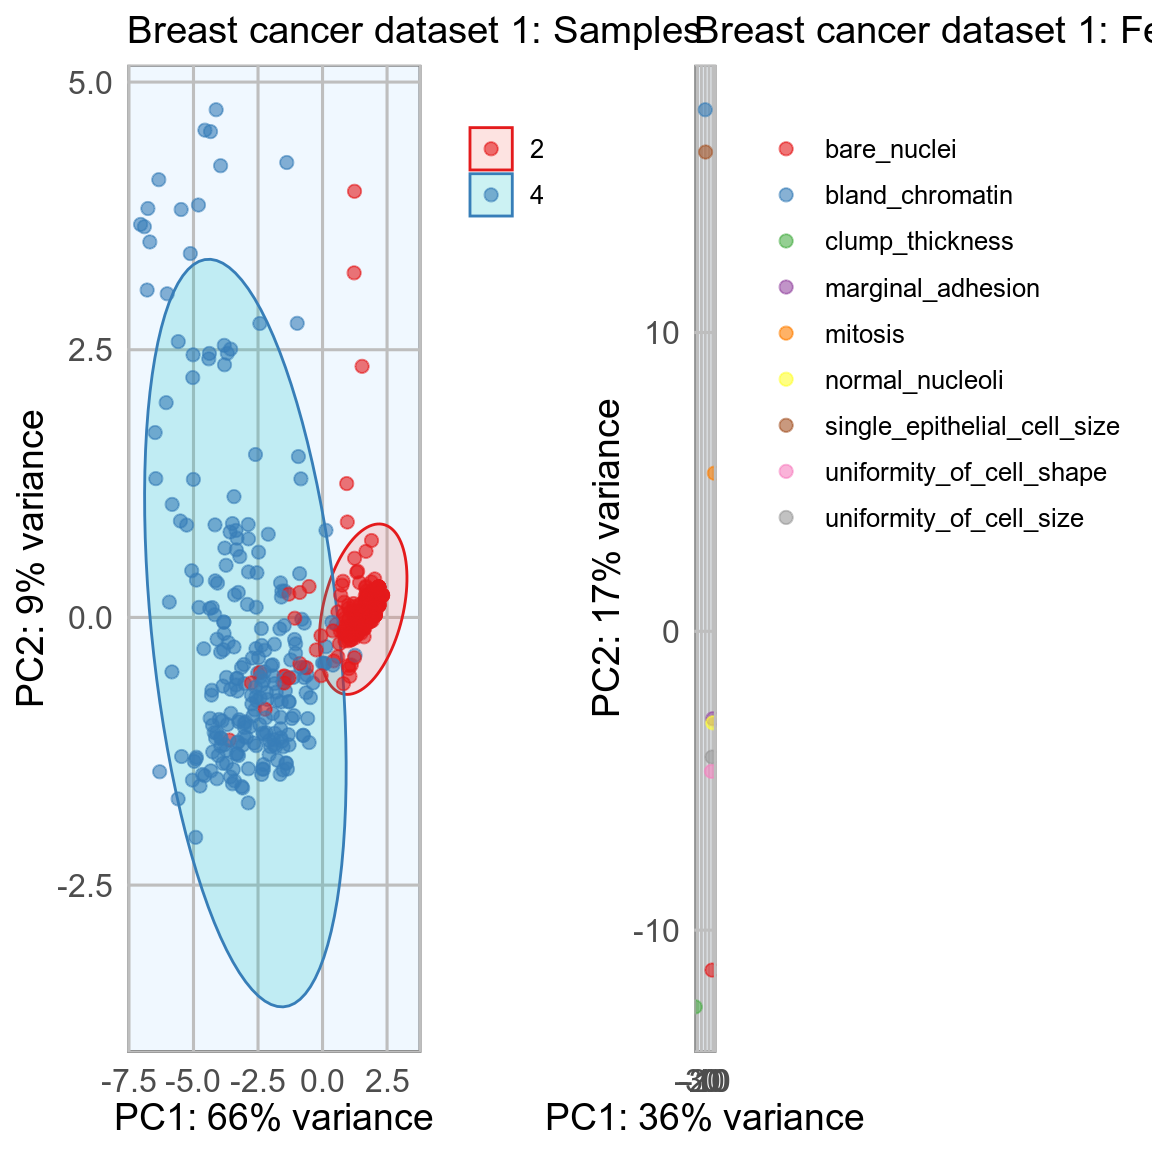
\includegraphics{DataAnalysis11_files/figure-latex/unnamed-chunk-12-1.pdf}

\begin{Shaded}
\begin{Highlighting}[]
\KeywordTok{plot}\NormalTok{(p2)}
\end{Highlighting}
\end{Shaded}

\includegraphics{DataAnalysis11_files/figure-latex/unnamed-chunk-12-2.pdf}

\begin{Shaded}
\begin{Highlighting}[]
\NormalTok{h_}\DecValTok{1}\NormalTok{ <-}\StringTok{ }\KeywordTok{hclust}\NormalTok{(}\KeywordTok{dist}\NormalTok{(}\KeywordTok{t}\NormalTok{(diagnosis_data[, }\DecValTok{2}\OperatorTok{:}\DecValTok{10}\NormalTok{]), }\DataTypeTok{method =} \StringTok{"euclidean"}\NormalTok{), }\DataTypeTok{method =} \StringTok{"complete"}\NormalTok{)}
\KeywordTok{plot}\NormalTok{(h_}\DecValTok{1}\NormalTok{)}
\end{Highlighting}
\end{Shaded}

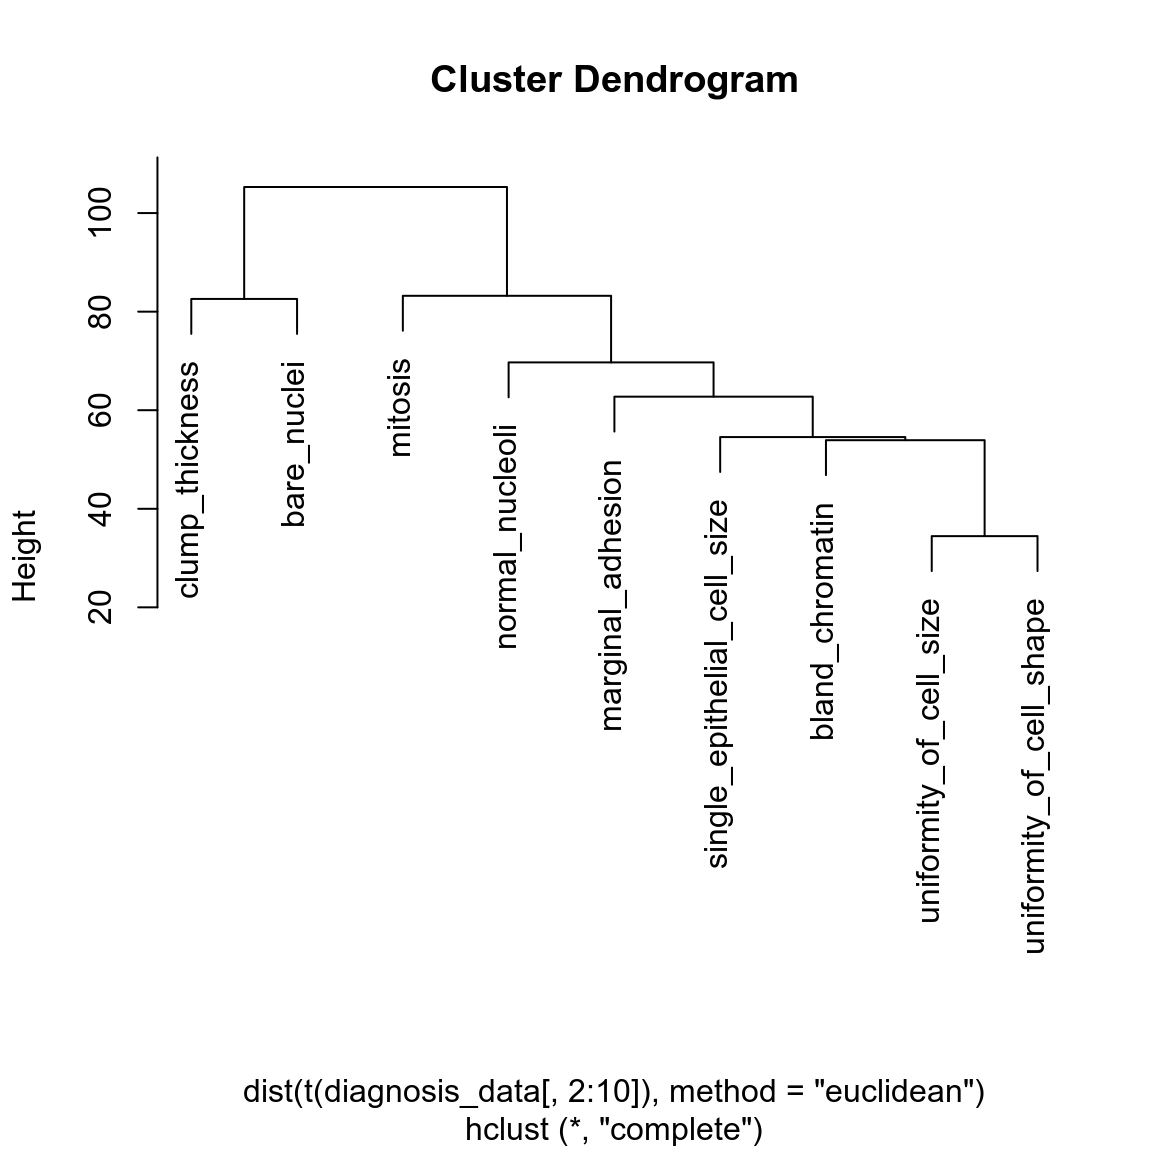
\includegraphics{DataAnalysis11_files/figure-latex/unnamed-chunk-13-1.pdf}

\begin{Shaded}
\begin{Highlighting}[]
\KeywordTok{library}\NormalTok{(tidyr)}
\end{Highlighting}
\end{Shaded}

\begin{verbatim}
## 
## Attaching package: 'tidyr'
\end{verbatim}

\begin{verbatim}
## The following object is masked from 'package:S4Vectors':
## 
##     expand
\end{verbatim}

\begin{verbatim}
## The following object is masked from 'package:mice':
## 
##     complete
\end{verbatim}

\begin{Shaded}
\begin{Highlighting}[]
\NormalTok{diagnosis_data_gather <-}\StringTok{ }\NormalTok{diagnosis_data }\OperatorTok
\StringTok{  }\KeywordTok{gather}\NormalTok{(measure, value, clump_thickness}\OperatorTok{:}\NormalTok{mitosis)}

\KeywordTok{ggplot}\NormalTok{(}\DataTypeTok{data =}\NormalTok{ diagnosis_data_gather, }\KeywordTok{aes}\NormalTok{(}\DataTypeTok{x =}\NormalTok{ value, }\DataTypeTok{fill =}\NormalTok{ classes, }\DataTypeTok{color =}\NormalTok{ classes)) }\OperatorTok{+}
\StringTok{  }\KeywordTok{geom_density}\NormalTok{(}\DataTypeTok{alpha =} \FloatTok{0.3}\NormalTok{, }\DataTypeTok{size =} \DecValTok{1}\NormalTok{) }\OperatorTok{+}
\StringTok{  }\KeywordTok{geom_rug}\NormalTok{() }\OperatorTok{+}
\StringTok{  }\KeywordTok{scale_fill_brewer}\NormalTok{(}\DataTypeTok{palette =} \StringTok{"Set1"}\NormalTok{) }\OperatorTok{+}
\StringTok{  }\KeywordTok{scale_color_brewer}\NormalTok{(}\DataTypeTok{palette =} \StringTok{"Set1"}\NormalTok{) }\OperatorTok{+}
\StringTok{  }\KeywordTok{facet_wrap}\NormalTok{( }\OperatorTok{~}\StringTok{ }\NormalTok{measure, }\DataTypeTok{scales =} \StringTok{"free_y"}\NormalTok{, }\DataTypeTok{ncol =} \DecValTok{3}\NormalTok{)}
\end{Highlighting}
\end{Shaded}

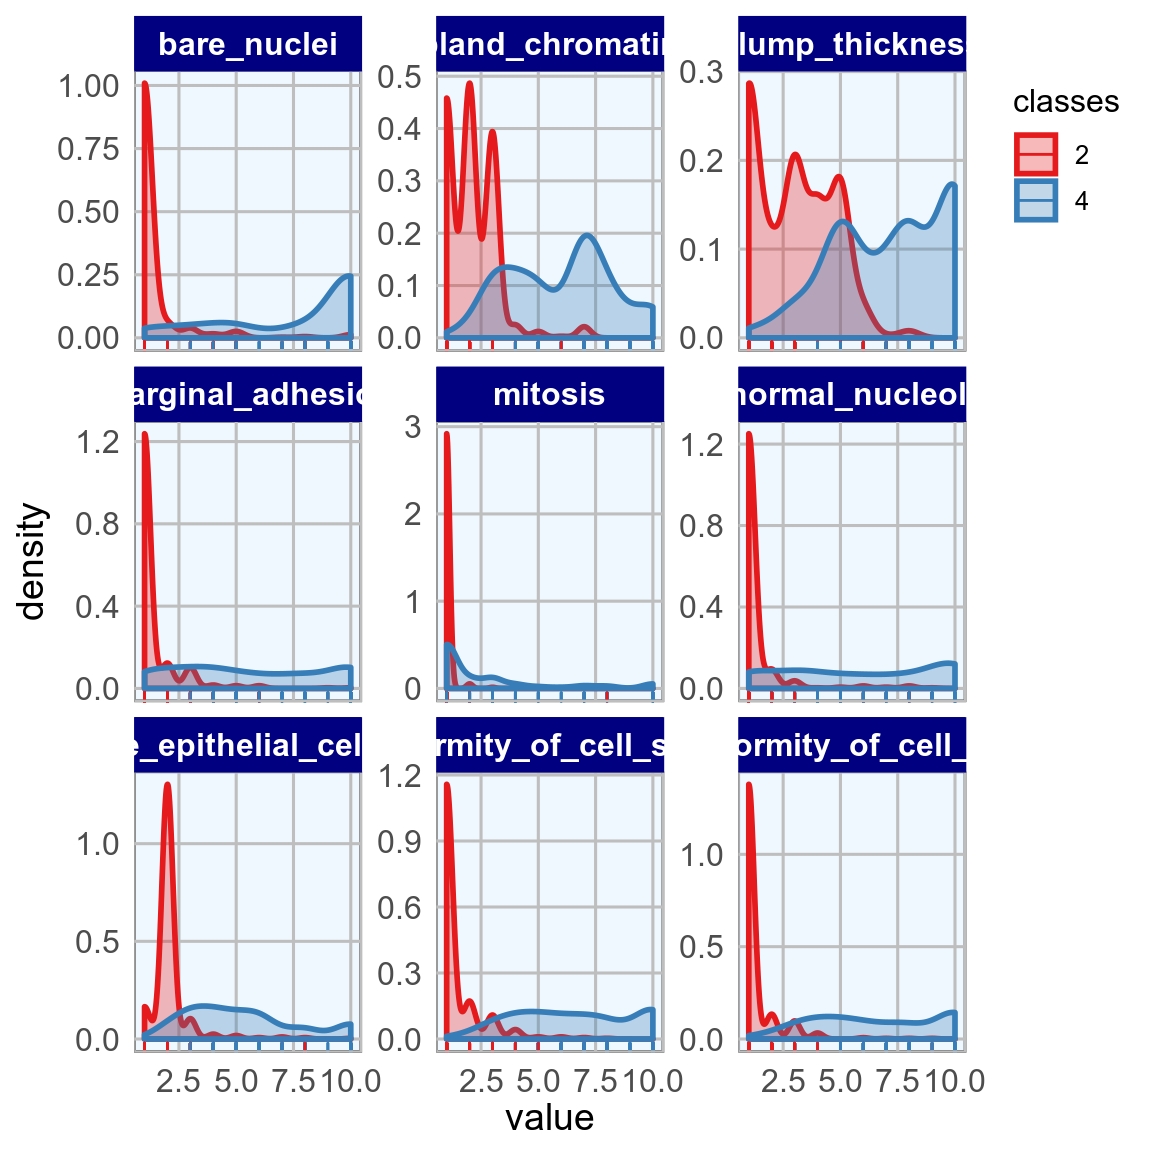
\includegraphics{DataAnalysis11_files/figure-latex/unnamed-chunk-14-1.pdf}

\begin{Shaded}
\begin{Highlighting}[]
\NormalTok{p1 <-}\StringTok{ }\KeywordTok{pca_func}\NormalTok{(}\DataTypeTok{data =} \KeywordTok{t}\NormalTok{(diagnosis_data_}\DecValTok{2}\NormalTok{[, }\DecValTok{3}\OperatorTok{:}\DecValTok{32}\NormalTok{]), }\DataTypeTok{groups =} \KeywordTok{as.character}\NormalTok{(diagnosis_data_}\DecValTok{2}\OperatorTok{$}\NormalTok{diagnosis), }\DataTypeTok{title =} \StringTok{"Breast cancer dataset 2: Samples"}\NormalTok{)}
\NormalTok{p2 <-}\StringTok{ }\KeywordTok{pca_func}\NormalTok{(}\DataTypeTok{data =}\NormalTok{ diagnosis_data_}\DecValTok{2}\NormalTok{[, }\DecValTok{3}\OperatorTok{:}\DecValTok{32}\NormalTok{], }\DataTypeTok{groups =} \KeywordTok{as.character}\NormalTok{(}\KeywordTok{colnames}\NormalTok{(diagnosis_data_}\DecValTok{2}\NormalTok{[, }\DecValTok{3}\OperatorTok{:}\DecValTok{32}\NormalTok{])), }\DataTypeTok{title =} \StringTok{"Breast cancer dataset 2: Features"}\NormalTok{, }\DataTypeTok{print_ellipse =} \OtherTok{FALSE}\NormalTok{)}
\KeywordTok{plot}\NormalTok{(p1)}
\end{Highlighting}
\end{Shaded}

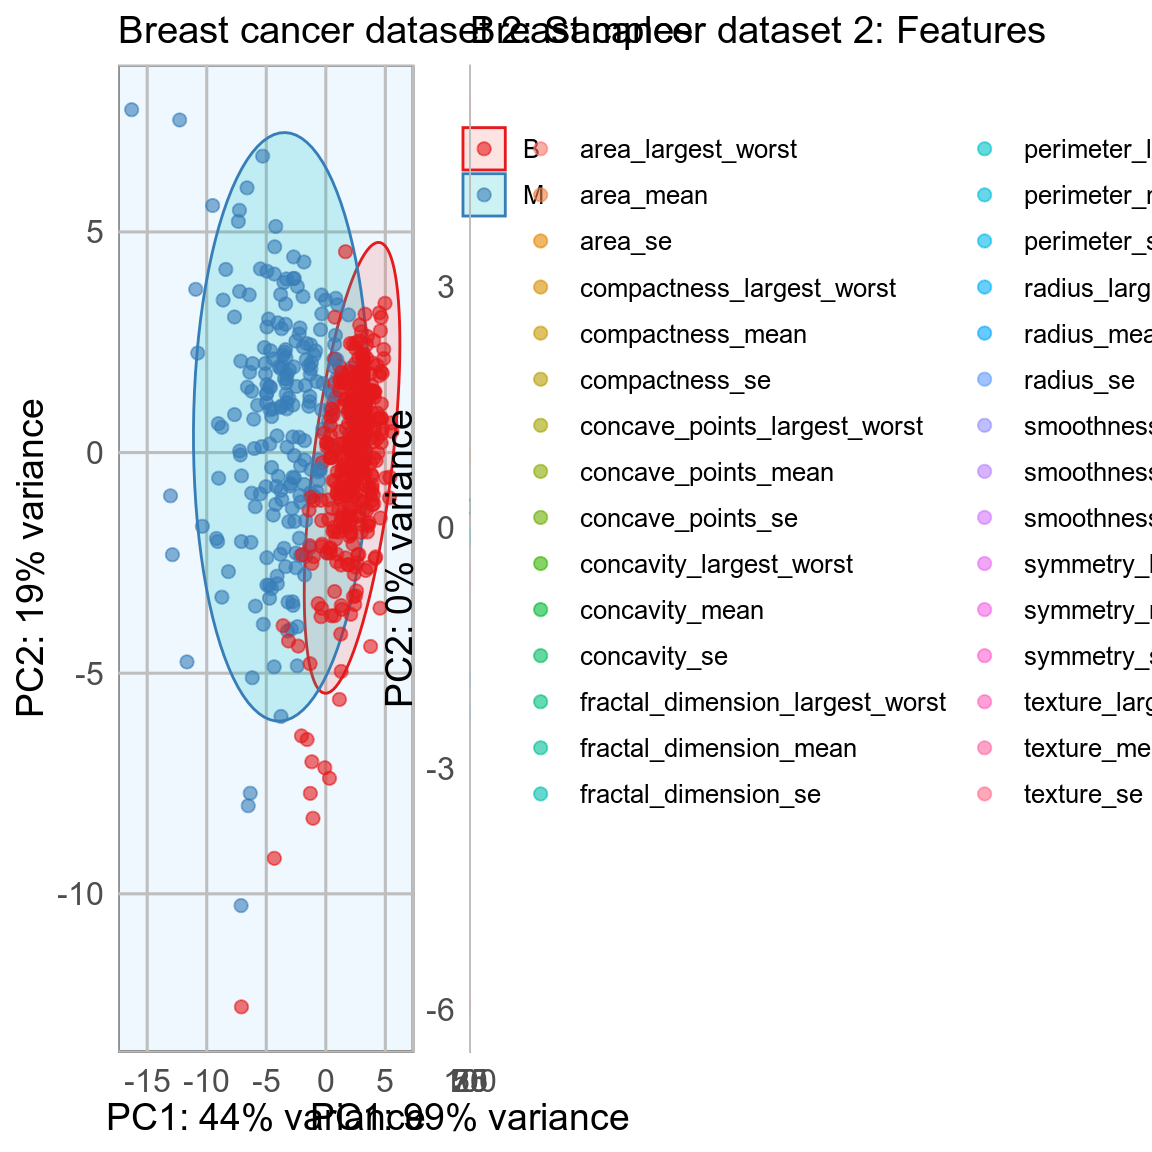
\includegraphics{DataAnalysis11_files/figure-latex/unnamed-chunk-15-1.pdf}

\begin{Shaded}
\begin{Highlighting}[]
\KeywordTok{plot}\NormalTok{(p2)}
\end{Highlighting}
\end{Shaded}

\includegraphics{DataAnalysis11_files/figure-latex/unnamed-chunk-15-2.pdf}

\begin{Shaded}
\begin{Highlighting}[]
\NormalTok{h_}\DecValTok{2}\NormalTok{ <-}\StringTok{ }\KeywordTok{hclust}\NormalTok{(}\KeywordTok{dist}\NormalTok{(}\KeywordTok{t}\NormalTok{(diagnosis_data_}\DecValTok{2}\NormalTok{[, }\DecValTok{3}\OperatorTok{:}\DecValTok{32}\NormalTok{]), }\DataTypeTok{method =} \StringTok{"euclidean"}\NormalTok{), }\DataTypeTok{method =} \StringTok{"complete"}\NormalTok{)}
\KeywordTok{plot}\NormalTok{(h_}\DecValTok{2}\NormalTok{)}
\end{Highlighting}
\end{Shaded}

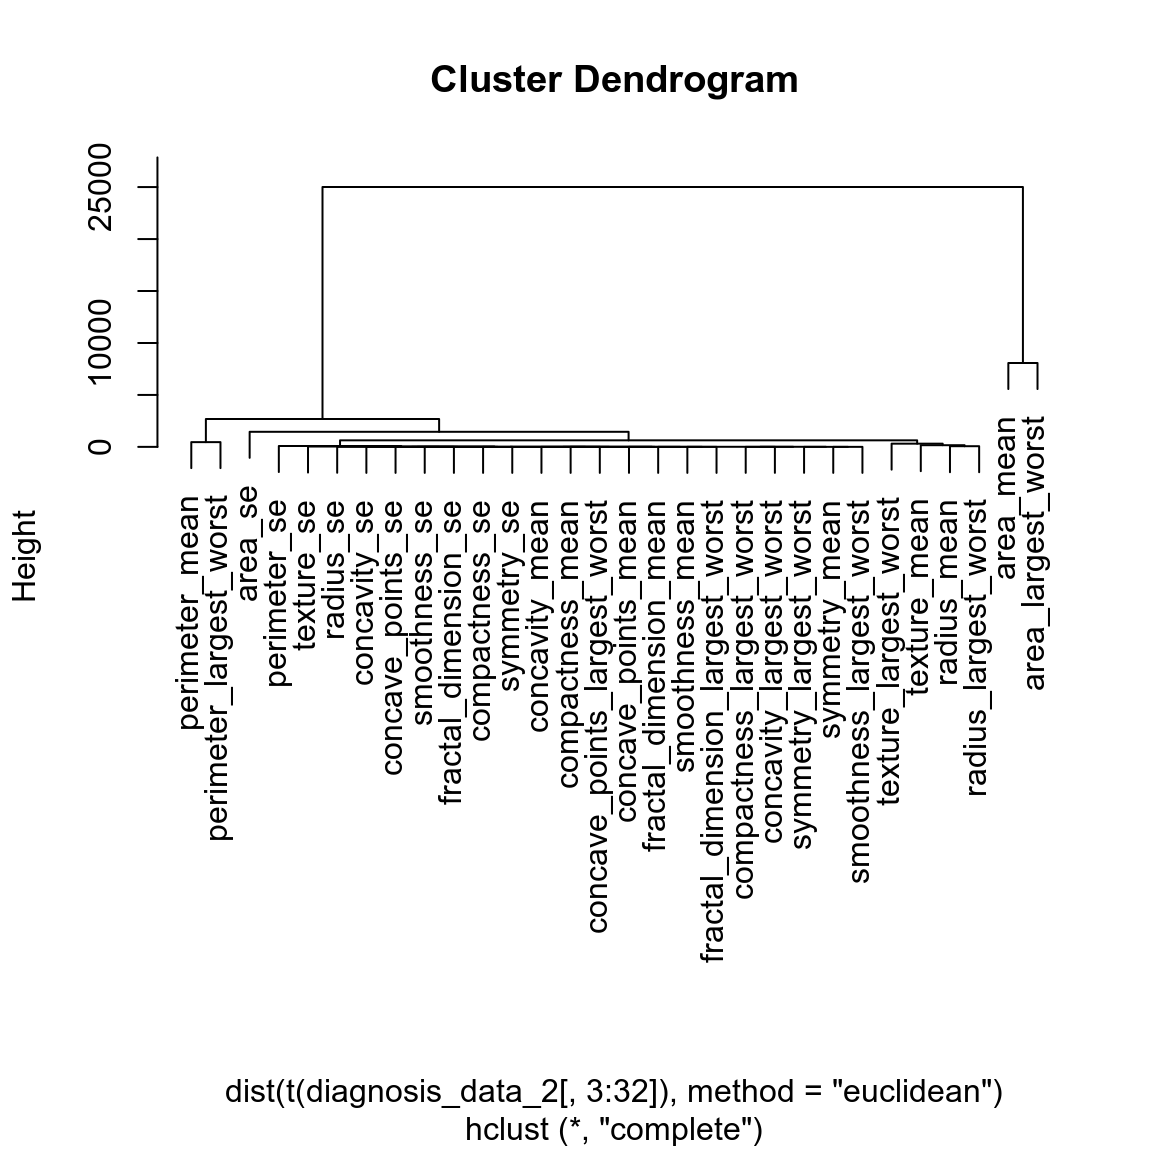
\includegraphics{DataAnalysis11_files/figure-latex/unnamed-chunk-16-1.pdf}

\begin{Shaded}
\begin{Highlighting}[]
\NormalTok{p1 <-}\StringTok{ }\KeywordTok{pca_func}\NormalTok{(}\DataTypeTok{data =} \KeywordTok{t}\NormalTok{(diagnosis_data_}\DecValTok{3}\NormalTok{[, }\DecValTok{2}\OperatorTok{:}\DecValTok{34}\NormalTok{]), }\DataTypeTok{groups =} \KeywordTok{as.character}\NormalTok{(diagnosis_data_}\DecValTok{3}\OperatorTok{$}\NormalTok{outcome), }\DataTypeTok{title =} \StringTok{"Breast cancer dataset 3: Samples"}\NormalTok{)}
\NormalTok{p2 <-}\StringTok{ }\KeywordTok{pca_func}\NormalTok{(}\DataTypeTok{data =}\NormalTok{ diagnosis_data_}\DecValTok{3}\NormalTok{[, }\DecValTok{2}\OperatorTok{:}\DecValTok{34}\NormalTok{], }\DataTypeTok{groups =} \KeywordTok{as.character}\NormalTok{(}\KeywordTok{colnames}\NormalTok{(diagnosis_data_}\DecValTok{3}\NormalTok{[, }\DecValTok{2}\OperatorTok{:}\DecValTok{34}\NormalTok{])), }\DataTypeTok{title =} \StringTok{"Breast cancer dataset 3: Features"}\NormalTok{, }\DataTypeTok{print_ellipse =} \OtherTok{FALSE}\NormalTok{)}
\KeywordTok{plot}\NormalTok{(p1)}
\end{Highlighting}
\end{Shaded}

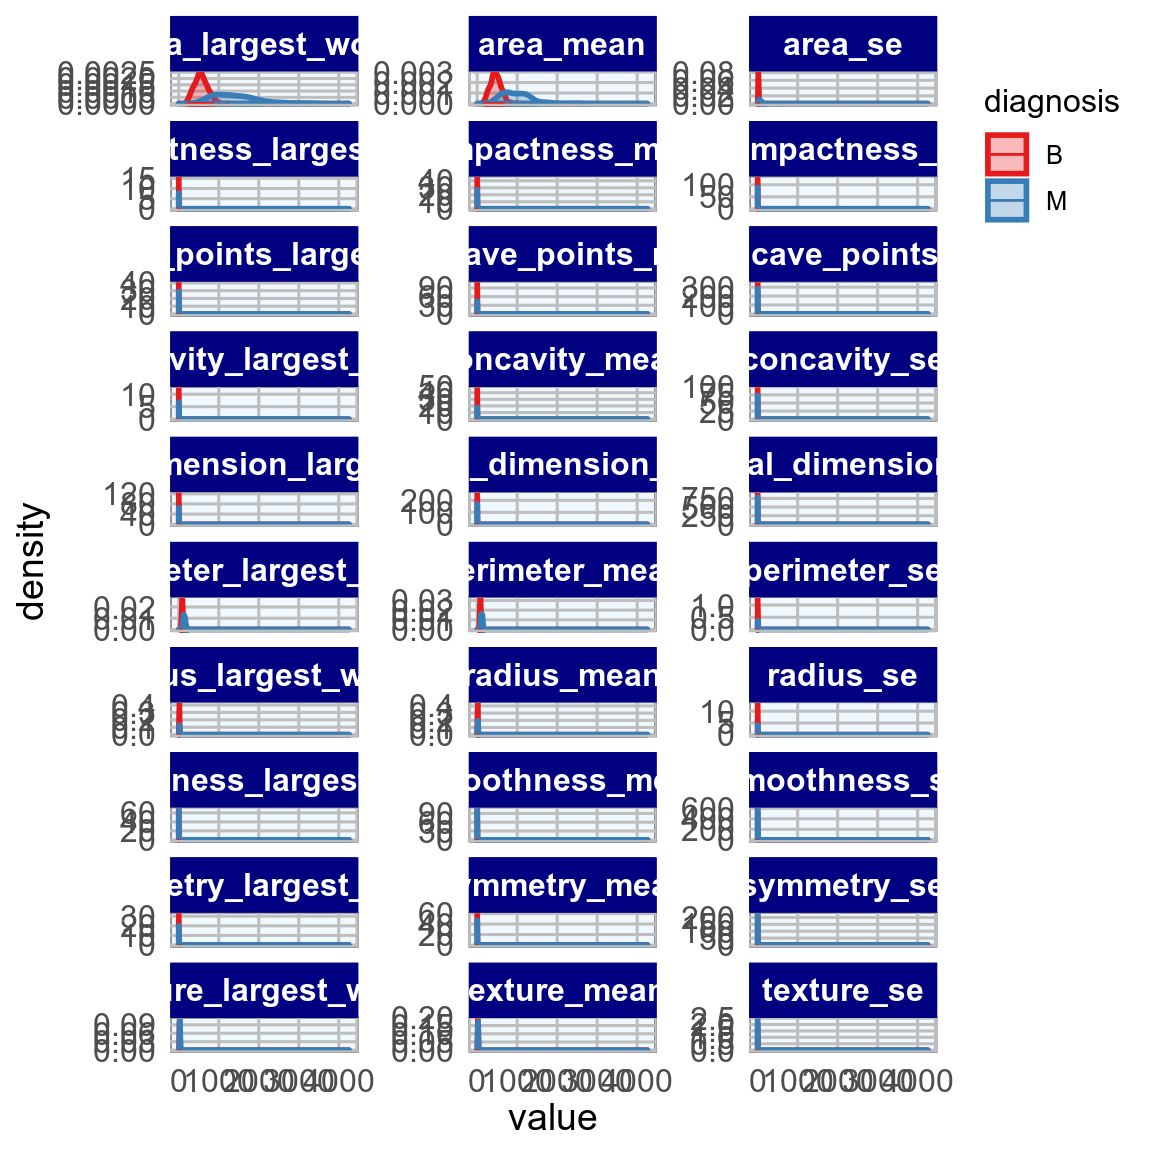
\includegraphics{DataAnalysis11_files/figure-latex/unnamed-chunk-17-1.pdf}

\begin{Shaded}
\begin{Highlighting}[]
\KeywordTok{plot}\NormalTok{(p2)}
\end{Highlighting}
\end{Shaded}

\includegraphics{DataAnalysis11_files/figure-latex/unnamed-chunk-17-2.pdf}

\begin{Shaded}
\begin{Highlighting}[]
\NormalTok{h_}\DecValTok{3}\NormalTok{ <-}\StringTok{ }\KeywordTok{hclust}\NormalTok{(}\KeywordTok{dist}\NormalTok{(}\KeywordTok{t}\NormalTok{(diagnosis_data_}\DecValTok{3}\NormalTok{[,}\DecValTok{2}\OperatorTok{:}\DecValTok{34}\NormalTok{]), }\DataTypeTok{method =} \StringTok{"euclidean"}\NormalTok{), }\DataTypeTok{method =} \StringTok{"complete"}\NormalTok{)}
\KeywordTok{plot}\NormalTok{(h_}\DecValTok{3}\NormalTok{)}
\end{Highlighting}
\end{Shaded}

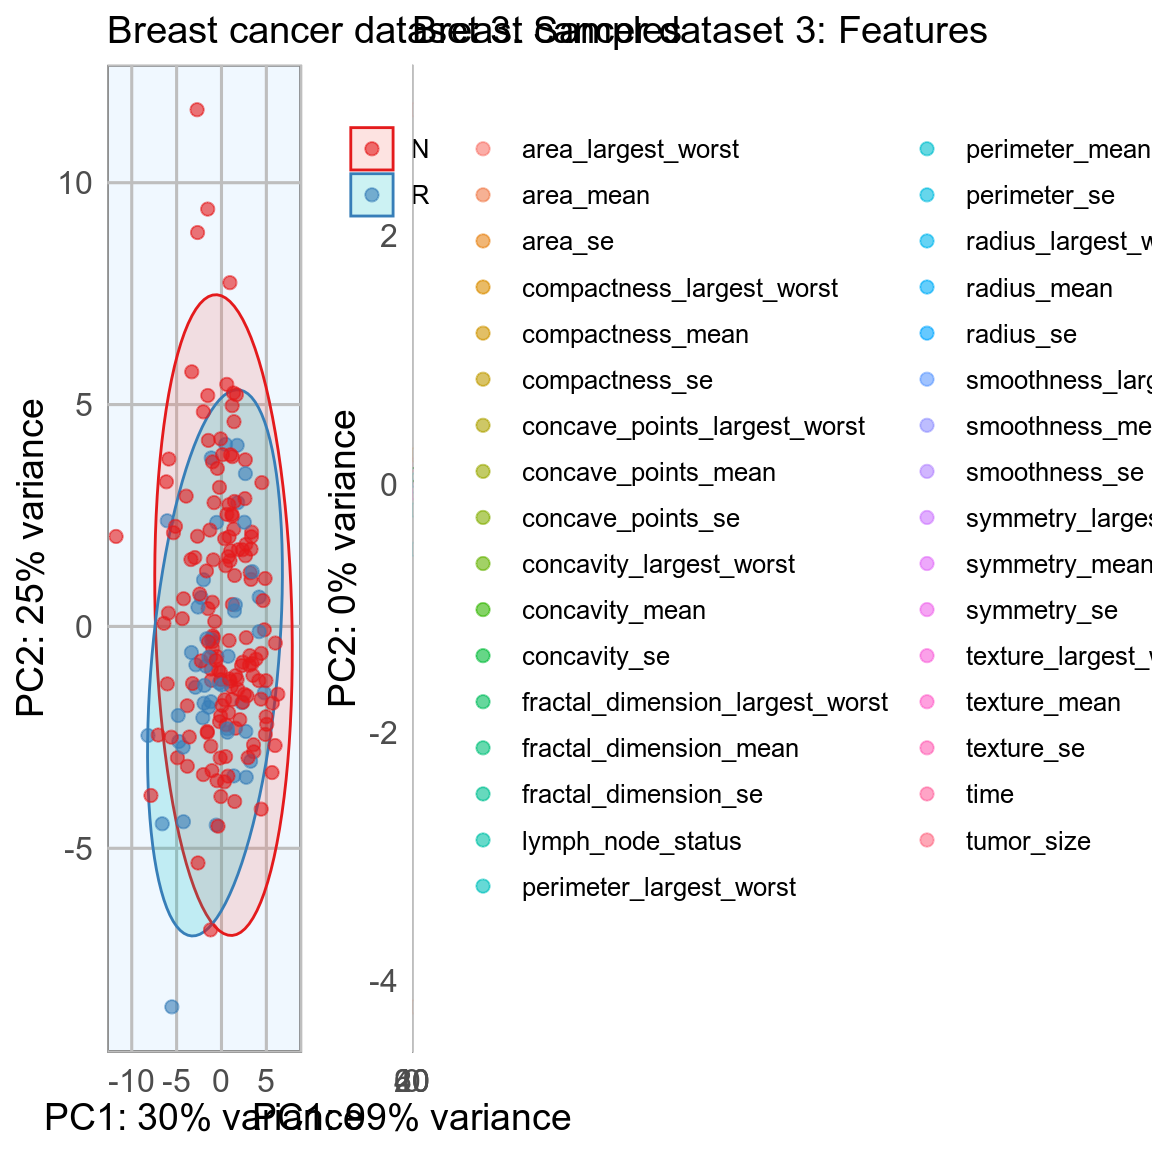
\includegraphics{DataAnalysis11_files/figure-latex/unnamed-chunk-18-1.pdf}

\begin{Shaded}
\begin{Highlighting}[]
\CommentTok{# parallel processing}
\KeywordTok{registerDoParallel}\NormalTok{()}

\CommentTok{# prepare training scheme}
\NormalTok{control <-}\StringTok{ }\KeywordTok{trainControl}\NormalTok{(}\DataTypeTok{method =} \StringTok{"repeatedcv"}\NormalTok{, }\DataTypeTok{number =} \DecValTok{10}\NormalTok{, }\DataTypeTok{repeats =} \DecValTok{10}\NormalTok{)}

\NormalTok{feature_imp <-}\StringTok{ }\ControlFlowTok{function}\NormalTok{(model, title) \{}
  
  \CommentTok{# estimate variable importance}
\NormalTok{  importance <-}\StringTok{ }\KeywordTok{varImp}\NormalTok{(model, }\DataTypeTok{scale =} \OtherTok{TRUE}\NormalTok{)}
  
  \CommentTok{# prepare dataframes for plotting}
\NormalTok{  importance_df_}\DecValTok{1}\NormalTok{ <-}\StringTok{ }\NormalTok{importance}\OperatorTok{$}\NormalTok{importance}
\NormalTok{  importance_df_}\DecValTok{1}\OperatorTok{$}\NormalTok{group <-}\StringTok{ }\KeywordTok{rownames}\NormalTok{(importance_df_}\DecValTok{1}\NormalTok{)}
  
\NormalTok{  importance_df_}\DecValTok{2}\NormalTok{ <-}\StringTok{ }\NormalTok{importance_df_}\DecValTok{1}
\NormalTok{  importance_df_}\DecValTok{2}\OperatorTok{$}\NormalTok{Overall <-}\StringTok{ }\DecValTok{0}
  
\NormalTok{  importance_df <-}\StringTok{ }\KeywordTok{rbind}\NormalTok{(importance_df_}\DecValTok{1}\NormalTok{, importance_df_}\DecValTok{2}\NormalTok{)}
  
\NormalTok{  plot <-}\StringTok{ }\KeywordTok{ggplot}\NormalTok{() }\OperatorTok{+}
\StringTok{    }\KeywordTok{geom_point}\NormalTok{(}\DataTypeTok{data =}\NormalTok{ importance_df_}\DecValTok{1}\NormalTok{, }\KeywordTok{aes}\NormalTok{(}\DataTypeTok{x =}\NormalTok{ Overall, }\DataTypeTok{y =}\NormalTok{ group, }\DataTypeTok{color =}\NormalTok{ group), }\DataTypeTok{size =} \DecValTok{2}\NormalTok{) }\OperatorTok{+}
\StringTok{    }\KeywordTok{geom_path}\NormalTok{(}\DataTypeTok{data =}\NormalTok{ importance_df, }\KeywordTok{aes}\NormalTok{(}\DataTypeTok{x =}\NormalTok{ Overall, }\DataTypeTok{y =}\NormalTok{ group, }\DataTypeTok{color =}\NormalTok{ group, }\DataTypeTok{group =}\NormalTok{ group), }\DataTypeTok{size =} \DecValTok{1}\NormalTok{) }\OperatorTok{+}
\StringTok{    }\KeywordTok{theme}\NormalTok{(}\DataTypeTok{legend.position =} \StringTok{"none"}\NormalTok{) }\OperatorTok{+}
\StringTok{    }\KeywordTok{labs}\NormalTok{(}
      \DataTypeTok{x =} \StringTok{"Importance"}\NormalTok{,}
      \DataTypeTok{y =} \StringTok{""}\NormalTok{,}
      \DataTypeTok{title =}\NormalTok{ title,}
      \DataTypeTok{subtitle =} \StringTok{"Scaled feature importance"}\NormalTok{,}
      \DataTypeTok{caption =} \StringTok{"}\CharTok{\textbackslash{}n}\StringTok{Determined with Random Forest and}
\StringTok{      repeated cross validation (10 repeats, 10 times)"}
\NormalTok{    )}
  
  \KeywordTok{return}\NormalTok{(plot)}
  
\NormalTok{\}}
\end{Highlighting}
\end{Shaded}

\begin{Shaded}
\begin{Highlighting}[]
\CommentTok{# train the model}
\KeywordTok{set.seed}\NormalTok{(}\DecValTok{27}\NormalTok{)}
\NormalTok{imp_}\DecValTok{1}\NormalTok{ <-}\StringTok{ }\KeywordTok{train}\NormalTok{(classes }\OperatorTok{~}\StringTok{ }\NormalTok{., }\DataTypeTok{data =}\NormalTok{ diagnosis_data, }\DataTypeTok{method =} \StringTok{"rf"}\NormalTok{, }\DataTypeTok{preProcess =} \KeywordTok{c}\NormalTok{(}\StringTok{"scale"}\NormalTok{, }\StringTok{"center"}\NormalTok{), }\DataTypeTok{trControl =}\NormalTok{ control)}
\NormalTok{p1 <-}\StringTok{ }\KeywordTok{feature_imp}\NormalTok{(imp_}\DecValTok{1}\NormalTok{, }\DataTypeTok{title =} \StringTok{"Breast cancer dataset 1"}\NormalTok{)}
\KeywordTok{set.seed}\NormalTok{(}\DecValTok{27}\NormalTok{)}
\NormalTok{imp_}\DecValTok{2}\NormalTok{ <-}\StringTok{ }\KeywordTok{train}\NormalTok{(diagnosis }\OperatorTok{~}\StringTok{ }\NormalTok{., }\DataTypeTok{data =}\NormalTok{ diagnosis_data_}\DecValTok{2}\NormalTok{[, }\OperatorTok{-}\DecValTok{1}\NormalTok{], }\DataTypeTok{method =} \StringTok{"rf"}\NormalTok{, }\DataTypeTok{preProcess =} \KeywordTok{c}\NormalTok{(}\StringTok{"scale"}\NormalTok{, }\StringTok{"center"}\NormalTok{), }\DataTypeTok{trControl =}\NormalTok{ control)}
\NormalTok{p2 <-}\StringTok{ }\KeywordTok{feature_imp}\NormalTok{(imp_}\DecValTok{2}\NormalTok{, }\DataTypeTok{title =} \StringTok{"Breast cancer dataset 2"}\NormalTok{)}
\KeywordTok{set.seed}\NormalTok{(}\DecValTok{27}\NormalTok{)}
\NormalTok{imp_}\DecValTok{3}\NormalTok{ <-}\StringTok{ }\KeywordTok{train}\NormalTok{(outcome }\OperatorTok{~}\StringTok{ }\NormalTok{., }\DataTypeTok{data =}\NormalTok{ diagnosis_data_}\DecValTok{3}\NormalTok{, }\DataTypeTok{method =} \StringTok{"rf"}\NormalTok{, }\DataTypeTok{preProcess =} \KeywordTok{c}\NormalTok{(}\StringTok{"scale"}\NormalTok{, }\StringTok{"center"}\NormalTok{), }\DataTypeTok{trControl =}\NormalTok{ control)}
\NormalTok{p3 <-}\StringTok{ }\KeywordTok{feature_imp}\NormalTok{(imp_}\DecValTok{3}\NormalTok{, }\DataTypeTok{title =} \StringTok{"Breast cancer dataset 3"}\NormalTok{)}
\KeywordTok{grid.arrange}\NormalTok{(p1, p2, p3, }\DataTypeTok{ncol =} \DecValTok{3}\NormalTok{, }\DataTypeTok{widths =} \KeywordTok{c}\NormalTok{(}\FloatTok{0.3}\NormalTok{, }\FloatTok{0.35}\NormalTok{, }\FloatTok{0.35}\NormalTok{))}
\end{Highlighting}
\end{Shaded}

\includegraphics{DataAnalysis11_files/figure-latex/unnamed-chunk-20-1.pdf}


\end{document}
